\newpage 
\numberwithin{equation}{section}
\section{Theoretical Framework}

\subsection{Plasma and Magnetic Confinement Fundamentals}

\subsubsection{Basic Plasma Parameters and the Confinement Criterion}
A plasma is a quasineutral ionized gas exhibiting collective behavior over characteristic system dimensions $L_{\mathrm{sys}} \gg \lambda_D$, where the Debye shielding length is $\lambda_D = \sqrt{\varepsilon_0 k_B T_e / (n_e e^2)}$ ($\mathrm{m}$), with vacuum permittivity $\varepsilon_0$ ($\mathrm{F/m}$), Boltzmann constant $k_B$ ($\mathrm{J/K}$), electron temperature $T_e$ ($\mathrm{K}$), electron density $n_e$ ($\mathrm{m^{-3}}$), and elementary charge $e$ ($\mathrm{C}$) \cite{chen2016introduction}. For $L_{\mathrm{sys}} \gg \lambda_D$, macroscopic quasineutrality yields $n_i \simeq n_e \simeq n$ ($\mathrm{m^{-3}}$), where $n_i$ and $n$ denote ion and bulk plasma densities, while collective electrostatic oscillations arise at the electron plasma angular frequency $\omega_{pe} = \sqrt{n_e e^2 / (m_e \varepsilon_0)}$ ($\mathrm{rad/s}$), with electron mass $m_e$ ($\mathrm{kg}$) \cite{chen2016introduction}. Self-sustained fusion additionally requires satisfying the Lawson triple-product criterion $n \tau_E T \ge 3 \times 10^{21}\,\mathrm{m^{-3}\cdot s\cdot keV}$, where $\tau_E$ is the energy confinement time ($\mathrm{s}$) and $T$ is expressed in thermal energy units $k_B T$ ($\mathrm{keV}$; $1\,\mathrm{keV} = 1.602 \times 10^{-16}\,\mathrm{J} \equiv 1.16 \times 10^{7}\,\mathrm{K}$) \cite{chen2016introduction}. Confinement efficiency is quantified by the ratio of kinetic to magnetic pressure $\beta$, defined in Eq.~(\ref{eqn:beta}) \cite{chen2016introduction}:
\begin{equation} 
\label{eqn:beta}
\beta = \frac{\sum_j n_j k_B T_j}{\frac{B^2}{2\mu_0}},
\end{equation}
\noindent where $n_j$ ($\mathrm{m^{-3}}$) and $T_j$ ($\mathrm{K}$) are the number density and thermodynamic temperature of species $j$, $B$ is the magnetic field magnitude ($\mathrm{T}$), and $\mu_0$ is the vacuum permeability ($\mathrm{H/m}$).

\subsubsection{MHD Equations and Equilibrium}
The ideal MHD framework models macroscopic plasma dynamics as a single perfectly conducting fluid coupled to Maxwell's equations via mass continuity, adiabatic state evolution, ideal Ohm's law, and Amp\`ere--Faraday induction \cite{zheng, chen2016introduction}. In the static equilibrium limit of vanishing bulk fluid velocity, magnetic Lorentz forces balance the kinetic thermal pressure gradient across nested flux surfaces as expressed in Eq.~(\ref{eqn:MHD_equilibrium}) \cite{zheng, chen2016introduction}:
\begin{equation}
\label{eqn:MHD_equilibrium}
\mathbf{J} \times \mathbf{B} = \nabla p,
\end{equation}
\noindent where $\mathbf{J}$ is the plasma current density ($\mathrm{A/m^2}$), $\mathbf{B}$ is the magnetic field vector ($\mathrm{T}$), and $p$ is the scalar thermal plasma pressure ($\mathrm{Pa}$). Perturbations to this equilibrium excite shear Alfv\'en waves propagating along magnetic field lines \cite{zheng, chen2016introduction}.

\subsection{The Heliotron J Device}
Heliotron~J is a helical-axis heliotron with a pole number $L=1$ and field period $M=4$ continuous helical coil, utilizing auxiliary toroidal and vertical field coils to generate vacuum rotational transform without requiring a net toroidal plasma current \cite{chen2016introduction, Miyazawa2023, Yamamoto_2020}. Plasma heating is provided by NBI, which injects non-Maxwellian fast ions that drive kinetic MHD instabilities, and $70\,\mathrm{GHz}$ ECH for localized electron resonance \cite{nagasaki2020heliotron}. Key diagnostics (Figure~\ref{fig:locations}) include toroidal and poloidal Mirnov arrays (MP1--MP4 and PMP1--PMP14) measuring boundary magnetic fluctuations, diamagnetic loops recording macroscopic stored energy $W_p$ ($\mathrm{J}$), and a 16-channel ECE radiometer tracking relative electron temperature perturbations \cite{nagasaki2020heliotron}. Specifically, each inductive Mirnov probe (effective area-turns $NA$, $\mathrm{m^2}$, and amplifier gain $G$) senses the time-varying poloidal or toroidal magnetic flux derivative via Faraday's law, producing an output voltage $V_{\mathrm{Mirnov}}(t) = -G\,(NA)\,\mathrm{d}\tilde{B}_\theta/\mathrm{d}t$ ($\mathrm{V}$). The diamagnetic loop measures the plasma-induced excluded toroidal magnetic flux $\Delta\Phi_{\mathrm{dia}}$ ($\mathrm{Wb}$) proportional to perpendicular kinetic pressure, from which macroscopic stored energy $W_p \propto B_0 \Delta\Phi_{\mathrm{dia}}$ ($\mathrm{J}$) is integrated \cite{nagasaki2020heliotron}. Meanwhile, the $2~\mathrm{mm}$ ($140~\mathrm{GHz}$) heterodyne microwave interferometer measures the line-integrated optical phase shift $\Delta\varphi_{\mathrm{int}} = [e^2 / (2\varepsilon_0 m_e c \omega_{\mathrm{probe}})] \int n_e\,\mathrm{d}l$ ($\mathrm{rad}$) across the plasma chord (with speed of light $c$ and probing angular frequency $\omega_{\mathrm{probe}}$) to yield the line-averaged electron density $n_e$ ($\mathrm{m^{-3}}$) \cite{chen2016introduction, nagasaki2020heliotron}.

\begin{figure}[H]
  \centering
  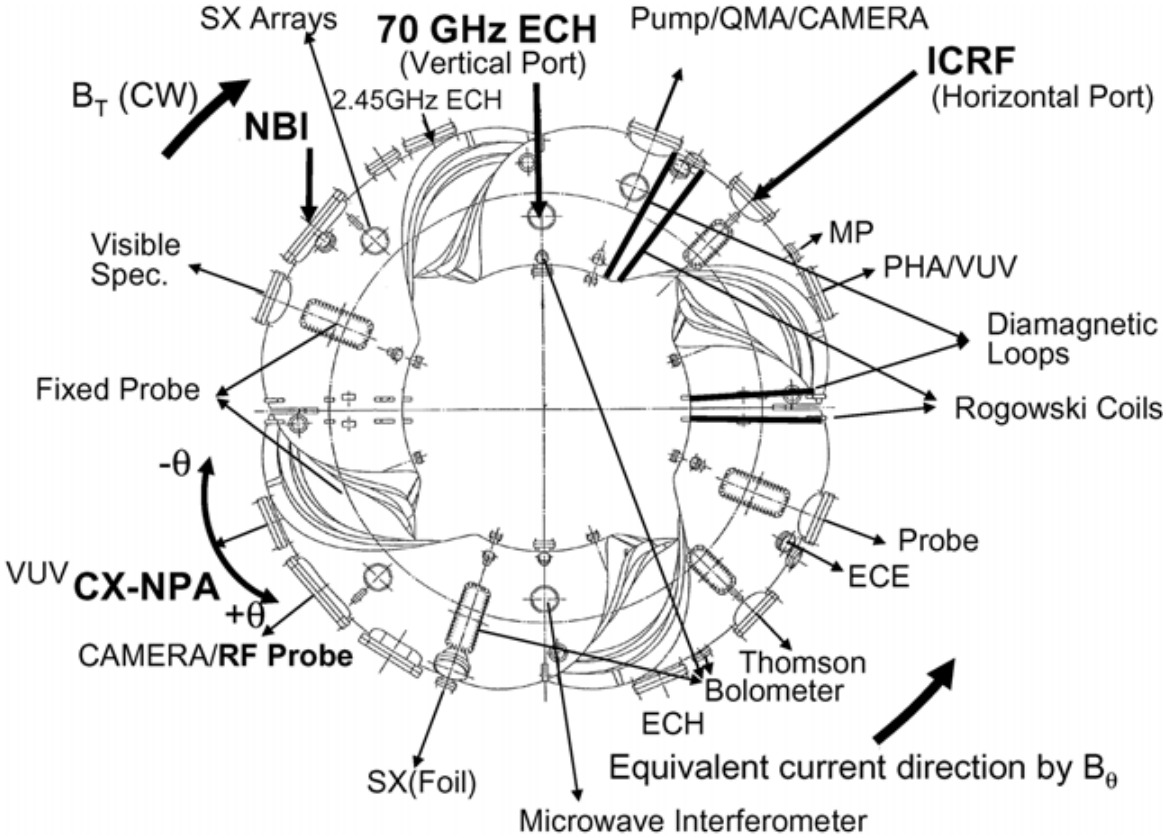
\includegraphics[width=0.7\textwidth]{Images/Locations.jpeg}
  \caption[Heating and diagnostic systems in Heliotron J]{Top-view schematic layout of the heating and diagnostic systems in Heliotron~J. Source: Okada et al.~\cite{Okada2007}.}
  \label{fig:locations}
\end{figure}

\subsection{MHD Instabilities and Alfv\'en Eigenmodes}

\subsubsection{Energetic-Particle-Driven Modes and State of the Art in Heliotron J}
Energetic particles (EPs) generated by NBI form an anisotropic velocity distribution whose free energy resonantly destabilizes shear Alfv\'en waves propagating at the Alfv\'en speed $v_A$ ($\mathrm{m/s}$) in Eq.~(\ref{eqn:alfven}) \cite{Heidbrink2008, Sheikh2023, Adulsiriswad_2024, Varela2015, chen2016introduction}:
\begin{equation}
\label{eqn:alfven}
v_A = \frac{B}{\sqrt{\mu_0 n_i m_i}},
\end{equation}
\noindent where $m_i$ is the ion mass ($\mathrm{kg}$). In three-dimensional heliotrons, periodic magnetic curvature couples poloidal and toroidal harmonics to open frequency gaps in the shear Alfv\'en continuum, sustaining weakly damped Alfv\'en eigenmodes (AEs) \cite{Varela2015, Adulsiriswad_2024}. Mode destabilization requires satisfying the wave--particle resonance condition in Eq.~(\ref{eqn:condition}) \cite{Adulsiriswad_2024}:
\begin{equation}
\label{eqn:condition}
\omega - n\omega_\phi + \ell\omega_\theta = 0,
\end{equation}
\noindent where $\omega$ is the mode angular frequency ($\mathrm{rad/s}$), $n$ is the toroidal mode number, $\omega_\phi$ and $\omega_\theta$ are the EP toroidal transit and poloidal drift frequencies ($\mathrm{rad/s}$), and $\ell$ is an integer bounce/transit harmonic. In flux coordinates $(\theta, \zeta)$, a coherent magnetic perturbation $\tilde{B}$ ($\mathrm{T}$) is decomposed into helical Fourier harmonics via Eq.~(\ref{eqn:periodicity}):
\begin{equation}
\label{eqn:periodicity}    
\tilde{B}(\theta, \zeta) \propto \exp\left[\mathrm{i}(m\theta - n\zeta)\right],
\end{equation}
\noindent where $m$ is the poloidal mode number, $\mathrm{i} = \sqrt{-1}$, and $\theta$ and $\zeta$ are the poloidal and toroidal angles ($\mathrm{rad}$). Continuum gap modes localize near rational flux surfaces where the rotational transform $\iota$ ($\mathrm{rad}$) satisfies Eq.~(\ref{eqn:varela}) \cite{Varela2015}:
\begin{equation}
\label{eqn:varela}
    \frac{\iota}{2\pi} = \frac{n}{m}.
\end{equation}

\noindent Away from exact rational surfaces, the local parallel wavenumber ($\mathrm{m^{-1}}$) is $k_\parallel = (m\iota/(2\pi) - n)/R_0$, where $R_0$ is the major radius ($\mathrm{m}$), while toroidicity-induced harmonic coupling opens the toroidal Alfv\'en eigenmode (TAE) continuum gap centered at $f_{\mathrm{TAE}} = (\iota/2\pi)v_A/(4\pi R_0)$ ($\mathrm{Hz}$) \cite{Heidbrink2008, chen2016introduction, Varela2015}.

In Heliotron~J, experimental observations and Finite Aspect Ratio 3D (FAR3d) gyrofluid and MHD modeling have demonstrated how NBI fast-ion pressure gradients, pitch-angle anisotropy, and three-dimensional magnetic shear govern the excitation of low-$n$ EPMs, BAEs, and global Alfv\'en eigenmodes (GAEs) across the $40\text{--}120~\mathrm{kHz}$ frequency band \cite{Yamamoto_2020, Varela2015, Varela2024, Zhong2024}. Configuration-dependent rotational transform ($\iota/2\pi$) and beam-deposition profiles separate core-localized modes ($m = 1\text{--}4$) from outer-gradient beam-driven BAE/GAE-band instabilities observed near $\rho \approx 0.86\text{--}0.91$ with $m = 6\text{--}8$ \cite{zang2019observation, Varela2023, Zhong2024}. Furthermore, localized ECH and electron cyclotron current drive (ECCD) actively stabilize or shift energetic-particle-driven branches by tailoring core electron temperature and $\iota/2\pi$ \cite{zang2019observation, Varela2023, Adulsiriswad_2024}. Analogous fast-ion Alfv\'enic regimes occur across helical and stellarator experiments, including ECCD stabilization of EPMs and TAEs in the Large Helical Device \cite{Yamamoto_2020, Varela2015}, NBI-driven Alfv\'en eigenmode destabilization controlled by rational-surface topology in the TJ-II stellarator \cite{Varela2017}, and coherent micro-fluctuation characterization via correlation diagnostics in Wendelstein~7-X \cite{KraemerFlecken2024}.

Beyond linear stability, higher-order bispectral and bicoherence techniques reveal nonlinear three-wave coupling that redistributes energy across frequency scales and links macroscopic MHD modes to cross-field transport. Fourier bicoherence measurements have established resonant mode--mode phase locking among Alfv\'enic instabilities in tokamaks \cite{Hou2019} as well as nonlinear coupling between broadband turbulence and coherent modes in toroidal confinement devices \cite{Fujisawa2021}. Specifically in Heliotron~J, bicoherence analyses during the high-confinement mode (H-mode) and across core sawtooth relaxations, in which periodic internal MHD crashes flatten central temperature profiles, demonstrate strong nonlinear coupling between low-frequency MHD modes, edge turbulence, and intermittent confinement degradation \cite{Kin2025, Miyashita2025}. Separating genuine quadratic phase locking from finite-sample variance is thus critical to distinguish coupled daughter harmonics from independent instabilities.

\subsubsection{Theoretical Frequency Scaling Models}
\label{subsubsec:scaling_models}
To identify the physical dispersion of observed modes, instantaneous frequency trajectories are evaluated against seven candidate scaling models \cite{Varela2024}. Ideal shear Alfv\'en dispersion scales inversely with the square root of density as defined in Eq.~(\ref{eqn:shear_alfven}):
\begin{equation}
\label{eqn:shear_alfven}
f_A(t) \propto \frac{v_A(t)}{q R_0} \propto \frac{B}{\sqrt{n_e(t)}},
\end{equation}
\noindent where $f_A(t)$ is the Alfv\'en frequency ($\mathrm{Hz}$), $B$ is the magnetic field magnitude ($\mathrm{T}$), and $q = 2\pi/\iota$ is the safety factor. BAEs and geodesic acoustic modes (GAMs) scale with the ion-acoustic velocity via electron temperature in Eq.~(\ref{eqn:gam}), while compressibility-coupled Alfv\'en--acoustic dispersion follows Eq.~(\ref{eqn:compressibility}):
\begin{equation}
\label{eqn:gam}
f_{\mathrm{BAE}}(t) \propto \sqrt{T_e(t)},
\end{equation}
\begin{equation}
\label{eqn:compressibility}
f(t) \propto \sqrt{\frac{C_1}{n_e(t)} + C_2 T_e(t)},
\end{equation}
\noindent where $f_{\mathrm{BAE}}(t)$ and $f(t)$ are the mode frequencies ($\mathrm{Hz}$) and $C_1, C_2$ are empirical coupling constants. Beam-driven EPMs locked to fast-ion pressure gradients or injection power $P_{\mathrm{NBI}}(t)$ ($\mathrm{W}$) follow Eqs.~(\ref{eqn:epm_density}) and (\ref{eqn:epm_drift}):
\begin{equation}
\label{eqn:epm_density}
f_{\mathrm{EPM}}(t) \propto \sqrt{\frac{P_{\mathrm{NBI}}(t)}{n_e(t)}},
\end{equation}
\begin{equation}
\label{eqn:epm_drift}
f_{\mathrm{EPM}}(t) \propto P_{\mathrm{NBI}}(t),
\end{equation}
\noindent where $f_{\mathrm{EPM}}(t)$ is the energetic-particle-mode frequency ($\mathrm{Hz}$).
Finally, frequency shifts driven by plasma-current-induced rotational transform variations $\Delta\bar{\iota} \propto \Delta I_p$ and finite-$\beta$ diamagnetic equilibrium modifications follow Eq.~(\ref{eqn:shift_macro}):
\begin{equation}
\label{eqn:shift_macro}
f(t) \propto I_p(t), \quad f(t) \propto W_p(t),
\end{equation}
\noindent where $I_p(t)$ is the toroidal plasma current ($\mathrm{A}$) and $W_p(t)$ is the diamagnetic stored energy ($\mathrm{J}$).

\subsection{Signal Processing for MHD Mode Characterization}

\subsubsection{Time-Frequency Analysis}
The spectral bin width $\Delta f$ ($\mathrm{Hz}$) of a short-time Fourier transform (STFT) with window duration $T$ ($\mathrm{s}$) is governed by the Rayleigh frequency resolution limit in Eq.~(\ref{eqn:freq_res}) \cite{proakis2021digital}:
\begin{equation}
\label{eqn:freq_res}
\Delta f = \frac{1}{T}.
\end{equation}
To resolve rapid frequency chirps without fixed-window time--frequency trade-offs \cite{boashash2015time}, the continuous wavelet transform (CWT) employs the complex Morlet mother wavelet $\psi(t)$ in Eq.~(\ref{eqn:morlet}) \cite{addison2016illustrated}:
\begin{equation}
\label{eqn:morlet}
\psi(t) = \pi^{-1/4} \mathrm{e}^{\mathrm{i} \omega_0 t} \mathrm{e}^{-\frac{t^2}{2}},
\end{equation}
\noindent where $t$ is the dimensionless scale-normalized time, $\mathrm{i} = \sqrt{-1}$, and $\omega_0$ is the dimensionless central frequency. Physical modes are isolated from background fluctuations via a dual gate requiring the power spectral density (PSD) $P(f, t)$ ($\mathrm{V^2/Hz}$) to exceed a $3\sigma$ quiescent pre-plasma baseline in Eq.~(\ref{eqn:dominance}) \cite{bendat2010random} while simultaneously exhibiting inter-probe magnitude-squared spatial coherence $\gamma_{xy}^2(f)$ in Eq.~(\ref{eqn:coherence}) \cite{KraemerFlecken2024, Singh2024}:
\begin{equation}
\label{eqn:dominance}
P(f, t) \ge \mu_{\mathrm{noise}}(f) + 3\sigma_{\mathrm{noise}}(f),
\end{equation}
\begin{equation}
\label{eqn:coherence}
\gamma_{xy}^2(f) = \frac{|P_{xy}(f)|^2}{P_{xx}(f) P_{yy}(f)},
\end{equation}
\noindent where $\mu_{\mathrm{noise}}(f)$ and $\sigma_{\mathrm{noise}}(f)$ are the baseline spectral mean and standard deviation ($\mathrm{V^2/Hz}$), and $P_{xy}(f)$, $P_{xx}(f)$, and $P_{yy}(f)$ are the cross- and auto-spectral densities ($\mathrm{V^2/Hz}$). Under independent Gaussian white noise across $N_{\mathrm{seg}}$ non-overlapping segments, the $95\,\%$ coherence significance floor $\gamma_{95}^2$ is given by Eq.~(\ref{eqn:noise_floor}) \cite{carter1973estimation}:
\begin{equation}
\label{eqn:noise_floor}
\gamma_{95}^2 = 1 - (0.05)^{1/(N_{\mathrm{seg}} - 1)}.
\end{equation}
Continuous frequency shifts across heating transitions are tracked without bin-discretization steps via the power-weighted spectral centroid $f_{\mathrm{centroid}}(t)$ ($\mathrm{Hz}$) over $[f_{\min}, f_{\max}]$ in Eq.~(\ref{eqn:spectral_centroid}) \cite{boashash2015time}:
\begin{equation}
\label{eqn:spectral_centroid}
f_{\mathrm{centroid}}(t) = \frac{\sum_{f \in [f_{\min}, f_{\max}]} f \, P(f, t)}{\sum_{f \in [f_{\min}, f_{\max}]} P(f, t)},
\end{equation}
\noindent where $f_{\min}$ and $f_{\max}$ denote the lower and upper spectral band limits ($\mathrm{Hz}$).

\subsubsection{Toroidal Mode Identification}
The toroidal mode number $n$ is determined from the cross-spectral phase difference $\Delta\phi_{ij}^{\mathrm{meas}}$ ($\mathrm{rad}$) between coplanar toroidal probes $x_i, x_j$ ($\mathrm{V}$) at mode frequency $f_0$ ($\mathrm{Hz}$) in Eq.~(\ref{eqn:meas_phase}) \cite{bendat2010random, Smith1971}:
\begin{equation}
\label{eqn:meas_phase}
\Delta\phi_{ij}^{\mathrm{meas}} = \arg\left[P_{x_i x_j}(f_0)\right].
\end{equation}
Comparing against the wrapped theoretical phase shift $\Delta\phi_{ij}^{\mathrm{theo}}(n)$ ($\mathrm{rad}$) for coil toroidal separation $\Delta\varphi_{ij}$ ($\mathrm{rad}$) in Eq.~(\ref{eqn:theo_phase}) \cite{strait2006, Seo2019TheEO}, the best-fit $n$ minimizes the root-mean-square error ($\mathrm{RMSE}(n)$) of the phase fit ($\mathrm{rad}$, reported in degrees in Chapter~\ref{sec:results}) across $N_{\mathrm{pairs}}$ probe pairs in Eq.~(\ref{eqn:rmse}) \cite{schittenhelm1997analysis}:
\begin{equation}
\label{eqn:theo_phase}
\Delta\phi_{ij}^{\mathrm{theo}}(n) = (n \Delta\varphi_{ij} + \pi) \pmod{2\pi} - \pi,
\end{equation}
\begin{equation}
\label{eqn:rmse}
\mathrm{RMSE}(n) = \sqrt{\frac{1}{N_{\mathrm{pairs}}} \sum_{(i,j)} \left(\Delta\phi_{ij}^{\mathrm{meas}} - \Delta\phi_{ij}^{\mathrm{theo}}(n)\right)^2}.
\end{equation}

\subsubsection{Radial Fluctuation Localization and Multi-Coil Cross-Correlation}
\label{subsubsec:theory_ece_radial}
Whereas Mirnov coils measure edge magnetic perturbations $\tilde{B}_\theta$ at the vacuum vessel, internal radial mode localization relies on local electron temperature fluctuations $\tilde{T}_e(\rho, t)$ measured by ECE radiometry in optically thick plasmas \cite{KraemerFlecken2024, luo2020measurement}. For second-harmonic extraordinary-mode (X2) propagation, the emitted microwave frequency $f_{\mathrm{ECE}}$ ($\mathrm{Hz}$) is proportional to the local magnetic field modulus $|B(\rho)|$ ($\mathrm{T}$) in Eq.~(\ref{eqn:ece_resonance}) \cite{chen2016introduction, nagasaki2020heliotron, luo2020measurement}:
\begin{equation}
\label{eqn:ece_resonance}
f_{\mathrm{ECE}} = 2 f_{ce} = \frac{e |B(\rho)|}{\pi m_e},
\end{equation}
\noindent where $f_{ce}$ is the fundamental electron cyclotron frequency ($\mathrm{Hz}$), $e$ is the elementary charge ($\mathrm{C}$), $m_e$ is the electron mass ($\mathrm{kg}$), $\rho = r/a$ is the normalized minor radius, $r$ is the local minor radius ($\mathrm{m}$), and $a = 0.170\,\mathrm{m}$ is the average plasma minor radius. Although the $L=1, M=4$ helical geometry is non-axisymmetric, the ECE antenna at corner-section port \#11.5 (toroidal angle $\phi = \pm 45^\circ$, where toroidal coil A produces a tokamak-like vertical $\mathrm{mod}\text{-}B$ profile) views an equatorial chord along which $|B|$ decreases monotonically from the inboard high-field side to the outboard low-field edge \cite{luo2020measurement, Weir2019}.

Three-dimensional microwave ray-tracing with the Tracing Visualization (\textsc{TRAVIS}) code for the standard configuration (helical-to-vertical coil current ratio $H + V = +89\,\%$, setting the standard vacuum rotational transform $\iota(0)/2\pi \approx 0.56$ at $B_0 \approx 1.25~\mathrm{T}$) parameterizes the equilibrium frequency-to-radius calibration for Heliotron~J port \#11.5 \cite{luo2020measurement, Weir2019} via a first-order exponential decay ($\mathrm{ExpDec1}$, $R^2 = 0.999\ 71$) in Eq.~(\ref{eqn:ece_travis_fit}) and its inverse in Eq.~(\ref{eqn:ece_freq_from_rho}):
\begin{equation}
\label{eqn:ece_travis_fit}
\rho(f) = A_1 \exp\left(-\frac{f}{t_1}\right) + y_0 = 22.290\ 09 \exp\left(-\frac{f}{30.623\ 89}\right) - 2.247\ 43,
\end{equation}
\begin{equation}
\label{eqn:ece_freq_from_rho}
f(\rho) = -t_1 \ln\left(\frac{\rho - y_0}{A_1}\right) = -30.623\ 89 \ln\left(\frac{\rho + 2.247\ 43}{22.290\ 09}\right),
\end{equation}
\noindent where $f$ is the ECE channel frequency ($\mathrm{GHz}$), $y_0 = -2.247\ 43 \pm 0.024\ 14$, $A_1 = 22.290\ 09 \pm 0.314\ 97$, and $t_1 = (30.623\ 89 \pm 0.331\ 98)\,\mathrm{GHz}$, placing the outboard edge ($\rho = 1.00$) at $58.99\,\mathrm{GHz}$, the magnetic axis ($\rho = 0.00$) at $70.26\,\mathrm{GHz}$, and the inboard edge ($\rho = -1.00$) at $88.29\,\mathrm{GHz}$. Because each heterodyne channel integrates over a finite intermediate-frequency (IF) bandwidth $\Delta f_{\mathrm{IF}} \approx 1.0\,\mathrm{GHz}$, each measurement samples a radial shell of width $\Delta \rho$ given by Eq.~(\ref{eqn:ece_radial_res}):
\begin{equation}
\label{eqn:ece_radial_res}
\Delta \rho \approx \left| \frac{\mathrm{d}\rho}{\mathrm{d}f} \right| \Delta f_{\mathrm{IF}} = \frac{A_1}{t_1} \exp\left(-\frac{f}{t_1}\right) \Delta f_{\mathrm{IF}} \approx 0.08\text{--}0.09,
\end{equation}
\noindent corresponding to a physical radial resolution $\Delta r \approx a \Delta \rho \approx (1.4\text{--}1.5)\,\mathrm{cm}$ for $a = 0.170\,\mathrm{m}$, where valid local temperature interpretation requires optically thick core emission ($\tau_{\mathrm{opt}} \gg 1$, $\rho < 0.60$) \cite{luo2020measurement}.

To verify that internal ECE fluctuations couple to the global boundary mode across all 18 Mirnov coils (MP1--MP4 and PMP1--PMP14), the normalized carrier cross-correlation $R_{\mathrm{car}}(\tau)$ evaluates fast phase-coherent coupling within $|\tau| \le 25\,\mu\mathrm{s}$ in Eq.~(\ref{eqn:xcorr_carrier}) \cite{Smith1971, bendat2010random}, while the Hilbert envelope cross-correlation $R_{\mathrm{env}}(\tau)$ captures wave-packet modulation across $|\tau| \le 100\,\mu\mathrm{s}$ in Eq.~(\ref{eqn:xcorr_envelope}) \cite{Fabus2021, boashash2015time}:
\begin{equation}
\label{eqn:xcorr_carrier}
R_{\mathrm{car}}(\tau) = \frac{\langle \tilde{T}_e(t) \tilde{B}_\theta(t+\tau) \rangle}{\sigma_{\tilde{T}} \sigma_{\tilde{B}}},
\end{equation}
\begin{equation}
\label{eqn:xcorr_envelope}
R_{\mathrm{env}}(\tau) = \frac{\langle [A_{\tilde{T}}(t) - \bar{A}_{\tilde{T}}] [A_{\tilde{B}}(t+\tau) - \bar{A}_{\tilde{B}}] \rangle}{\sigma_{A_{\tilde{T}}} \sigma_{A_{\tilde{B}}}},
\end{equation}
\noindent where $\tau$ is the time lag ($\mathrm{s}$), $\sigma_{\tilde{T}}$ and $\sigma_{\tilde{B}}$ are the bandpass-filtered signal standard deviations ($\mathrm{V}$), $\bar{A}_{\tilde{T}}, \bar{A}_{\tilde{B}}$ and $\sigma_{A_{\tilde{T}}}, \sigma_{A_{\tilde{B}}}$ are the temporal means and standard deviations ($\mathrm{V}$) of the Hilbert envelopes $A_{\tilde{T}}(t)$ and $A_{\tilde{B}}(t)$, and $\langle \cdot \rangle$ is the temporal averaging operator. Combined with cross-spectral coherence $\gamma_{\tilde{T}\tilde{B}}^2(f)$ (Eq.~(\ref{eqn:coherence})) against $\gamma_{95}^2$ (Eq.~(\ref{eqn:noise_floor})), these metrics quantify internal-to-external mode coupling. Evaluated between adjacent ECE channels, this dual formalism distinguishes microscopic wave phase progression from macroscopic energy transport: the carrier phase delay derived from the cross-spectral phase $\Delta\phi$ (Eq.~(\ref{eqn:meas_phase})) reflects the local phase velocity $v_{\mathrm{ph},r}$ or stationary radial eigenmode phase structure \cite{Smith1971, Weir2019}. By contrast, the Hilbert envelope lag from $R_{\mathrm{env}}(\tau)$ (Eq.~(\ref{eqn:xcorr_envelope})) tracks macroscopic wavepacket modulation, measuring the radial group velocity $v_{\mathrm{g},r}$ and cross-field energy propagation direction \cite{Fabus2021, boashash2015time}.

\subsection{Signal Conditioning and Correlation Analysis}

\subsubsection{Instantaneous Parameters and Envelope Dynamics}
To extract continuous mode trajectories without phase distortion, magnetic fluctuation signals $x(t)$ ($\mathrm{V}$) are conditioned with a maximally flat group-delay Bessel bandpass filter \cite{zang2019observation}. The complex analytic signal $z(t)$ is constructed via the Hilbert transform $\mathcal{H}\{x(t)\}$ to obtain the instantaneous amplitude envelope $A(t)$ ($\mathrm{V}$), unwrapped phase $\phi(t)$ ($\mathrm{rad}$), and Savitzky--Golay differentiated instantaneous frequency $f(t)$ ($\mathrm{Hz}$) in Eq.~(\ref{eqn:hilbert_inst}) \cite{boashash2015time, Fabus2021}:
\begin{equation}
\label{eqn:hilbert_inst}
z(t) = x(t) + \mathrm{i}\mathcal{H}\{x(t)\} = A(t)\mathrm{e}^{\mathrm{i}\phi(t)}, \qquad f(t) = \frac{1}{2\pi}\frac{\mathrm{d}\phi(t)}{\mathrm{d}t}.
\end{equation}
Active mode bursts are isolated against non-Gaussian background noise and transient spikes using the Gaussian-consistent median absolute deviation (MAD) estimator $\hat{\sigma}_{\mathrm{MAD}}$ ($\mathrm{V}$) in Eq.~(\ref{eqn:mad_sigma}) \cite{RousseeuwCroux1993, james2021statistical}:
\begin{equation}
\label{eqn:mad_sigma}
\hat{\sigma}_{\mathrm{MAD}} = 1.4826\,\mathrm{median}\!\left(\left|x(t) - \mathrm{median}(x)\right|\right).
\end{equation}

\subsubsection{Spatial Harmonic Decomposition and Poloidal Phase}
To resolve the poloidal mode number $m$ across the irregularly spaced PMP1--PMP14 array and suppress spatial aliasing \cite{Klein2008}, the spatial NUDFT is evaluated via Eq.~(\ref{eqn:nudft}) \cite{dutt1993fast}:
\begin{equation}
\label{eqn:nudft}
S_k = \frac{1}{N_{\mathrm{probes}}} \sum_{j=1}^{N_{\mathrm{probes}}} S_j \mathrm{e}^{-\mathrm{i} k \theta_j},
\end{equation}
\noindent where $S_k$ is the spatial spectral amplitude at poloidal wavenumber $k$ ($\mathrm{T/s}$), $N_{\mathrm{probes}}$ is the number of poloidal coils, and $S_j$ ($\mathrm{T/s}$) and $\theta_j$ ($\mathrm{rad}$) are the complex temporal Fourier component and poloidal angle of coil $j$. The cross-spectral poloidal phase $\phi_j$ ($\mathrm{rad}$) relative to reference probe $S_{\mathrm{ref}}$ with phase $\phi_{\mathrm{ref}}$ ($\mathrm{rad}$) is extracted via Eq.~(\ref{eqn:pol_phase}) \cite{Smith1971}, and directional phase clustering around candidate harmonic $m$ is quantified by the Mardia--Jupp circular concentration coefficient $r_{\mathrm{circ}}(m) \in [0, 1]$ in Eq.~(\ref{eqn:r_circ}) \cite{mardia2000directional}:
\begin{equation}
\label{eqn:pol_phase}
\phi_j = \arg\left[\langle S_j(f) S_{\mathrm{ref}}^*(f) \rangle\right] - \phi_{\mathrm{ref}},
\end{equation}
\begin{equation}
\label{eqn:r_circ}
r_{\mathrm{circ}}(m) = \frac{1}{N_{\mathrm{probes}}} \sqrt{\left(\sum_{j=1}^{N_{\mathrm{probes}}} \cos(\phi_j - m\theta_j)\right)^2 + \left(\sum_{j=1}^{N_{\mathrm{probes}}} \sin(\phi_j - m\theta_j)\right)^2}.
\end{equation}
Because the three-dimensional $L=1, M=4$ helical geometry breaks single-harmonic poloidal orthogonality and permits coexisting or coupled poloidal harmonics $(m_1, m_2)$, a multi-branch directional phase-residual extension of circular dispersion statistics \cite{mardia2000directional} assigns each probe to its closest resonant branch via Eq.~(\ref{eqn:dual_branch_phase}) with the dual-branch circular concentration $r_{\mathrm{circ}}(m_1, m_2)$ defined in Eq.~(\ref{eqn:r_circ_dual}):
\begin{equation}
\label{eqn:dual_branch_phase}
\Delta\phi_j(m_1, m_2) = \min_{\mu \in \{m_1, m_2\}} \left| \mathrm{atan2}\left(\sin(\phi_j - \mu \theta_j),\, \cos(\phi_j - \mu \theta_j)\right) \right|,
\end{equation}
\begin{equation}
\label{eqn:r_circ_dual}
r_{\mathrm{circ}}(m_1, m_2) = \frac{1}{N_{\mathrm{probes}}} \sqrt{\left(\sum_{j=1}^{N_{\mathrm{probes}}} \cos\Delta\phi_j(m_1, m_2)\right)^2 + \left(\sum_{j=1}^{N_{\mathrm{probes}}} \sin\Delta\phi_j(m_1, m_2)\right)^2},
\end{equation}
\noindent where values of $r_{\mathrm{circ}}$ approaching unity and small mean absolute phase residuals $\overline{|\Delta\phi|}$ indicate coherent spatial phase alignment across the array \cite{mardia2000directional}.

\subsubsection{Correlation and Statistical Significance}
Dynamic response delays between mode parameters and macroscopic plasma profiles are quantified via the normalized lagged cross-correlation $R_{xy}(\tau)$ at time lag $\tau$ ($\mathrm{s}$) across $N$ samples in Eq.~(\ref{eqn:lagged_corr}) \cite{bendat2010random, Zhong2024}:
\begin{equation}
\label{eqn:lagged_corr}
R_{xy}(\tau) = \frac{1}{N} \sum_{t} \left(\frac{x(t) - \bar{x}}{\sigma_x}\right)\left(\frac{y(t+\tau) - \bar{y}}{\sigma_y}\right),
\end{equation}
\noindent where $\bar{x}, \bar{y}$ and $\sigma_x, \sigma_y$ are the sample means and standard deviations of synchronized time series $x(t)$ and $y(t)$. Because serial autocorrelation in smoothed plasma profiles inflates Type~I error rates, the nominal sample size $N$ is reduced to the effective sample size $N_{\mathrm{eff}}$ via Bartlett's joint-autocorrelation formula in Eq.~(\ref{eqn:neff}) \cite{Afyouni2019, shumway2017time}:
\begin{equation}
\label{eqn:neff}
N_{\mathrm{eff}} = \frac{N}{1 + 2 \sum_{k=1}^{M} \rho_x(k)\rho_y(k)},
\end{equation}
\noindent where $\rho_x(k)$ and $\rho_y(k)$ are the sample autocorrelation function (ACF) values of $x(t)$ and $y(t)$ at lag $k$ up to maximum lag $M$. Hypothesis testing employs the autocorrelation-adjusted $t$-statistic in Eq.~(\ref{eqn:t_stat}) \cite{shumway2017time} and first-order partial correlation $r_{xy \cdot z}$ in Eq.~(\ref{eqn:partial_corr}) to control for shared step-function artifacts $z$ \cite{james2021statistical}:
\begin{equation}
\label{eqn:t_stat}
t = r \sqrt{\frac{N_{\mathrm{eff}} - 2 - n_{\mathrm{control}}}{1 - r^2}},
\end{equation}
\begin{equation}
\label{eqn:partial_corr}
r_{xy \cdot z} = \frac{r_{xy} - r_{xz}r_{yz}}{\sqrt{(1 - r_{xz}^2)(1 - r_{yz}^2)}},
\end{equation}
\noindent where $r, r_{xy}, r_{xz}, r_{yz}$ are pairwise Pearson correlation coefficients and $n_{\mathrm{control}}$ is the number of control variables. Family-wise error across $m$ simultaneous tests is controlled via the Bonferroni threshold $\alpha_{\mathrm{adj}}$ in Eq.~(\ref{eq:bonferroni}) \cite{dunn1961multiple} alongside Benjamini--Hochberg false discovery rate (FDR-BH) adjustments \cite{Benjamini1995}:
\begin{equation}
\label{eq:bonferroni}
\alpha_{\mathrm{adj}} = \frac{\alpha}{m},
\end{equation}
\noindent where $m$ is the number of simultaneous hypothesis tests and $\alpha$ is the nominal significance level.

\subsection{Higher-Order Spectral Analysis for Nonlinear Wave Coupling}

\subsubsection{Bicoherence and Coupling Domains}
Quadratic nonlinear three-wave coupling is quantified via the auto-bispectrum $B(f_1, f_2)$ ($\mathrm{V^3/Hz^3}$) in Eq.~(\ref{eqn:bispectrum}) and the normalized squared auto-bicoherence $b^2(f_1, f_2) \in [0, 1]$ in Eq.~(\ref{eqn:bicoherence}) \cite{proakis2021digital, Hou2019, Fujisawa2021}:
\begin{equation}
\label{eqn:bispectrum}
B(f_1, f_2) = \langle X(f_1) X(f_2) X^*(f_1 \pm f_2) \rangle,
\end{equation}
\begin{equation}
\label{eqn:bicoherence}
b^2(f_1, f_2) = \frac{|\langle X(f_1) X(f_2) X^*(f_1 \pm f_2) \rangle|^2}{\langle |X(f_1) X(f_2)|^2 \rangle \langle |X(f_1 \pm f_2)|^2 \rangle},
\end{equation}
\noindent where $X(f)$ is the segmented complex Fourier spectrum ($\mathrm{V/Hz}$) at interacting frequencies $f_1, f_2$ ($\mathrm{Hz}$), $\langle \cdot \rangle$ is the expectation across $N_{\mathrm{ensemble}}$ segments, and $*$ denotes complex conjugation. Under a Gaussian null hypothesis, the significance threshold $b^2_\alpha$ at level $\alpha$ is approximated by Eq.~(\ref{eqn:b2_stat}) \cite{Hou2019, Fujisawa2021, HinichWolinsky2005}:
\begin{equation}
\label{eqn:b2_stat}
b^2_\alpha = -\frac{\ln(\alpha)}{N_{\mathrm{ensemble}}}.
\end{equation}
To eliminate bispectral permutation redundancies while maintaining positive physical frequencies ($f_1 > 0, f_2 > 0$), resonant triads are partitioned into sum-coupling (up-conversion) and difference-coupling (parametric decay / difference interaction) domains in Eqs.~(\ref{eqn:sum_domain}) and (\ref{eqn:diff_domain}):
\begin{equation}
\label{eqn:sum_domain}
f_3 = f_1 + f_2 \quad (f_1 > 0,\; f_2 > 0),
\end{equation}
\begin{equation}
\label{eqn:diff_domain}
f_3 = |f_1 - f_2| \quad (\text{or } f_1 - f_2 = f_3 \text{ with } f_1 > f_2 > 0),
\end{equation}
\noindent where $f_3$ is the coupled frequency ($\mathrm{Hz}$) bounded by the Nyquist limit; in the general bispectral notation $B(f_1, f_2) = \langle X(f_1) X(f_2) X^*(f_1 + f_2) \rangle$, a positive-frequency difference triad $f_a - f_b = f_c$ corresponds to setting $f_2 = -f_b$ via Hermitian symmetry $X(-f_b) = X^*(f_b)$.

\subsubsection{Bias Scaling, Convergence Extrapolation, and Empirical Benchmarking}
Because finite-sample bicoherence estimators carry positive bias ($\mathrm{E}[\hat{b}^2] \approx 1/N_{\mathrm{ensemble}}$) \cite{HinichWolinsky2005}, candidate transition shifts and triads in heated windows \cite{Kin2025, Miyashita2025} are benchmarked against $N_{\mathrm{null}}$ null realizations via the Davison--Hinkley empirical $p$-value ($p_{\mathrm{emp}}$) in Eq.~(\ref{eqn:empirical_p}) \cite{DavisonHinkley1997, james2021statistical}:
\begin{equation}
\label{eqn:empirical_p}
p_{\mathrm{emp}} = \frac{k + 1}{N_{\mathrm{null}} + 1},
\end{equation}
\noindent where $k$ is the count of null realizations equaling or exceeding the observed statistic. To separate genuine quadratic phase locking from $O(1/K)$ finite-sample bias across $K$ averaged segments, the sub-ensemble convergence trajectory $b^2(K)$ is regressed linearly against $1/K$ and extrapolated to the infinite-ensemble limit ($1/K \to 0$) via Eq.~(\ref{eqn:b2_convergence}) \cite{KimPowers1979, HinichWolinsky2005}:
\begin{equation}
\label{eqn:b2_convergence}
b^2(K) = b_0 + \frac{C}{K},
\end{equation}
\noindent where $b_0 = b^2_\infty$ is the asymptotic squared bicoherence intercept and $C$ is the finite-sample bias slope. Chronological non-stationarities are suppressed by averaging $N_{\mathrm{sub}}$ random sub-ensembles sampled without replacement over $K \in [K_{\mathrm{min}}, 0.9\,N_{\mathrm{seg}}]$ (where $K_{\mathrm{min}}$ is the minimum averaged sub-ensemble size and $N_{\mathrm{seg}}$ is the total segment count), extracting $95\,\%$ confidence bounds $[q_{2.5}, q_{97.5}]$ defined as the $2.5\text{th}$ and $97.5\text{th}$ empirical percentiles of the sub-ensemble intercept distribution. Finally, $b_0$ is calibrated against $N_{\mathrm{null}}$ Fourier phase-randomized surrogates ($\phi_k \sim \mathcal{U}[0, 2\pi)$) preserving the exact sample PSD under $H_0: b^2_{\mathrm{pop}} = 0$, yielding the surrogate significance $p_{\mathrm{surr}}$ via Eq.~(\ref{eqn:empirical_p}).